% Autore originale della traduzione: Fabio Tempera
% Licenza della traduzione: MIT
% Manuale utente italiano della famiglia TESS.
% I dati numerici, gli autori e gli URL coincidono con i manuali originali
% citati nel capitolo 7. Non inventare figure: le fotografie tess-w.png e
% tess-4c.png sono le stesse già usate nei documenti CieloBuio, con citazione
% STARS4ALL/GUAIX.

\documentclass[11pt,a4paper]{report}

\usepackage{packages}

\title{Manuale utente TESS\\[0.6em]
\large Famiglia TESS-W, TESS-4C, TESS-P e TAS}
\author{Traduzione italiana: Fabio Tempera}
\date{}

\begin{document}

\maketitle

\begin{abstract}
Questo fascicolo traduce in italiano i manuali d'uso della famiglia di fotometri TESS (Telescope Encoder and Sky Sensor) sviluppati nell'ambito del progetto europeo STARS4ALL e del laboratorio LICA dell'Universidad Complutense de Madrid. Il nucleo operativo per una stazione fissa di rete è TESS-W; il modello a 4 canali TESS-4C (indicato anche come TESS-W4C) è lo strumento di riferimento per i nodi CieloBuio. TESS-P e TAS coprono le misure portatili e le mappe a scansione. I dati numerici, i nomi degli autori originali, gli URL e le indicazioni di licenza dei testi fonte sono riportati nel testo e nel capitolo~\ref{cap:fonti}. La traduzione è di Fabio Tempera.
\end{abstract}

\tableofcontents

\chapter{Introduzione}

Il fotometro TESS-W è uno strumento scientifico pensato per misurare in continuo, da una posizione fissa, l'evoluzione della brillanza del cielo notturno su molte notti consecutive. La calibrazione assoluta è eseguita presso il Laboratorio de Instrumentación Científica Avanzada dell'Universidad Complutense de Madrid (LICA-UCM). I risultati di calibrazione sono inviati all'utente in un rapporto separato.

La versione inglese di riferimento del manuale TESS-W è la 3.0 del maggio 2019, autori Lucía García (\texttt{lucia\_garcia@ucm.es}), Jaime Zamorano (\texttt{jzamoran@ucm.es}) e Carlos Tapia (\texttt{carloseugeniotapia@ucm.es}). Il testo inglese indica come sede aggiornata \url{http://tess.stars4all.eu/manual/}. Il file PDF UCM usato per questa traduzione è \url{https://guaix.fis.ucm.es/sites/guaix.fis.ucm.es.tess/files/documents/2020-06-v3_TESS-W_manual_english.pdf}. Il manuale inglese deriva da un originale in spagnolo di Cristóbal García, \url{http://www.observatorioremoto.com/tess/tess.pdf} (l'URL storico restituisce 404 al momento della traduzione; esiste ancora \url{http://www.observatorioremoto.com/TESS.pdf}, manuale TESS del 30 maggio 2016, che descrive il modo locale, encoder e nubi).

La guida rapida TESS-W versione 1.0 del maggio 2022, autore Jaime Zamorano, aggiorna i nomi SSID, i passi della pagina web interna e il controllo su Grafana. Per TESS-4C le fonti operative sono la pagina GUAIX \url{https://guaix.fis.ucm.es/tess/TESS-4C}, il blog STARS4ALL Photometers \url{https://tessskysensor.blogspot.com/2021/10/tess-w4c.html} e il foglio di montaggio \url{http://observatorioremoto.com/Mounting\%20TESS-W4C\%20v2.pdf} (9 dicembre 2022). TESS-P User Manual versione 2.1 (10 marzo 2021, changelog 10 maggio 2022) e TAS User Manual versione 2.4 (15 maggio 2024) sono di Cristóbal García, progetto STARS4ALL.

I PDF originali non sommano 17 pagine. TESS-W inglese 3.0 ha 12 pagine, la guida rapida 3, TESS-P 21, TAS 28, TESS 2016 22, il foglio di montaggio TESS-W4C alcune pagine di fotografie. Molte di quelle pagine sono schermate e illustrazioni. Questo fascicolo traduce per intero i dati operativi di TESS-W e TESS-4C e le sezioni operative di TESS-P e TAS, senza riprodurre ogni schermata originale.

La Figura~\ref{fig:tessw} mostra un esemplare TESS-W (stessa larghezza 0,55 usata nei documenti CieloBuio). La Figura~\ref{fig:tess4c} mostra un esemplare TESS-4C a larghezza piena di colonna, come nei medesimi documenti.

\begin{figure}[ht!]
\centering
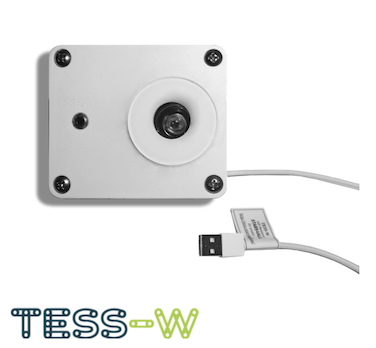
\includegraphics[width=0.55\textwidth]{figures/tess-w.png}
\caption{Fotometro TESS-W. Fonte: STARS4ALL / GUAIX-UCM.}
\label{fig:tessw}
\end{figure}

\begin{figure}[ht!]
\centering
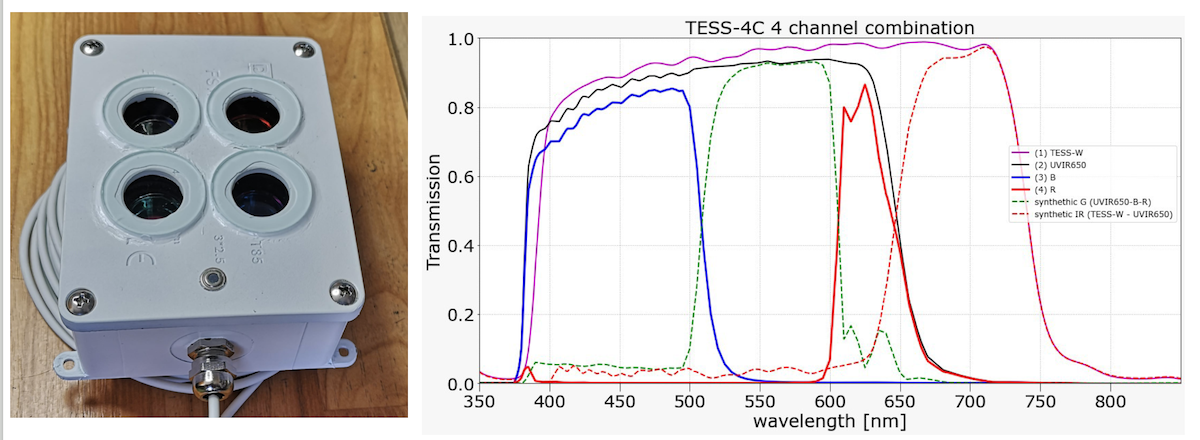
\includegraphics[width=\textwidth]{figures/tess-4c.png}
\caption{Fotometro TESS-4C (TESS-W4C). Fonte: STARS4ALL / GUAIX-UCM.}
\label{fig:tess4c}
\end{figure}

\chapter{TESS-W: installazione e configurazione}

\section{Informazioni generali}

Per funzionare in modo corretto la stazione va installata in un punto elevato, di preferenza su un tetto, con una presa di alimentazione e copertura WiFi per l'invio in tempo reale. TESS-W ha un connettore USB che consente l'alimentazione con un caricatore da telefono. Il caricatore va posto in una presa coperta e protetta dagli agenti atmosferici. È necessaria una sorgente in corrente continua da 5\,V.

L'intensità di corrente è compresa fra 50 e 100\,mA (a seconda del segnale WiFi) quando la temperatura ambiente è superiore a 10\,$^\circ$C. Per temperature $T < 10\,^\circ$C si attiva una resistenza che alza la temperatura interna, per evitare condensa sul finestrino e per fondere il gelo. In questa condizione la corrente è compresa fra 500 e 600\,mA. Il consumo di potenza varia quindi da 0,25\,W a 3\,W in funzione della temperatura esterna.

Dopo l'installazione il fotometro TESS-W entra nella rete di fotometri STARS4ALL. Le misure inviate sono archiviate in depositi ad accesso libero. La pagina \url{http://tess.stars4all.eu/} raccoglie i collegamenti per scaricare i file e per visualizzare i grafici dell'intera serie, comprese le misure in tempo reale.

TESS-W è pensato come stazione fissa di brillanza notturna e nuvolosità. La configurazione va completata prima del montaggio definitivo.

\section{Configurazione WiFi}

È necessaria una rete WiFi locale attiva perché il fotometro invii i dati. Una volta installato non richiede interventi: le misure partono in automatico verso il deposito.

La guida rapida del 2022 e il manuale 3.0 descrivono la stessa procedura, con nomi SSID aggiornati nel 2022.

Passo 1. Alla prima alimentazione TESS-W crea una propria rete WiFi. Nel manuale 3.0 il nome è \texttt{TESS-W}. Nella guida 2022, se il nome dello strumento è ad esempio \texttt{stars606}, l'SSID è \texttt{TESS-stars606}. Nel blog TESS-W4C l'SSID è del tipo \texttt{TESSW-starsxxx}. La rete è accessibile da computer o telefono senza password.

Passo 2. Dopo la connessione a quella rete si apre un browser all'indirizzo \url{http://192.168.4.1}.

Passo 3. Compare la schermata delle letture. Nel manuale 3.0 il collegamento da premere è ``Wi-Fi TESS Settings''. Nella guida 2022 e nel blog TESS-4C il pulsante è ``Show Settings''. Se la WiFi locale non è attiva alla prima accensione è necessario riavviare TESS-W.

Nelle versioni più recenti il nome del fotometro e il punto zero di calibrazione sono già memorizzati (esempio del manuale 3.0: \texttt{stars297} e $\mathrm{ZP}=20{,}46$).

Passo 4. I parametri, in minuscolo, sono i seguenti.

SSID: si seleziona la WiFi a cui il fotometro deve collegarsi.

Password: si inserisce la password di quella rete. Su una rete aperta, senza password, il blog TESS-4C indica di inserire comunque un valore, ad esempio 1234. Le reti pubbliche che richiedono un utente non sono adatte.

Name: il nome deve essere la parola \texttt{stars} in minuscolo seguita dal numero di serie. Non si usa ``Erase ALL Settings'' se non su indicazione dei gestori STARS4ALL; dopo la cancellazione il punto di accesso torna a chiamarsi \texttt{TESS-W} senza nome proprio.

Cons (punto zero): ogni fotometro ha il proprio valore. Il separatore decimale deve coincidere con quello del computer (punto o virgola).

Seg: frequenza di misura. Il valore da impostare è 60.

Tel.\ Port: porta di accesso locale, 23 per default.

Broker: per abilitare l'osservatorio remoto il server è \texttt{astrix.fis.ucm.es} (astrix, non asterix).

Nella guida 2022 di solito non è necessario cambiare la costante strumentale già inserita dopo la calibrazione. Il pulsante di invio sulla pagina 3 è etichettato ``enviar''.

Completata questa parte si stacca il fotometro dalla presa e lo si rialimenta dopo 30 secondi. TESS-W cerca l'SSID del router e inizia l'invio al broker.

Il controllo di presenza nella lista ``Sending Data'' con cuore verde è all'indirizzo \url{http://tess.stars4all.eu/plots/}. Se lo strumento è in ``Without data'' con cuore rosso spezzato, o non compare, si contattano i ricercatori UCM prima del montaggio definitivo. Indirizzo indicato nel manuale: \texttt{jzamorano@fis.ucm.es}.

La guida 2022 indica anche il cruscotto Grafana delle letture grezze:
\url{https://tess.dashboards.stars4all.eu/d/tess_raw/s4a-photometer-network-raw?orgId=1&refresh=1m&var-Tess=stars1}
dove \texttt{stars1} va sostituito con il nome dello strumento.

Per cambiare le impostazioni (ad esempio dopo una modifica della password WiFi) il fotometro va acceso in un ambiente in cui quella rete non è disponibile: si spegne il router, si inibisce il segnale, oppure si sposta lo strumento fuori portata. Alla pagina \url{http://192.168.4.1} compare un messaggio di reset. Dopo il reset si rientra nel menu ``WIFI Tess Settings''. Possono occorrere alcuni minuti perché lo strumento trovi la nuova rete.

Il livello di segnale WiFi ottimo, secondo il blog TESS-W4C, è compreso fra $-40$ e $-75$\,dBm. È molto basso a partire da $-85$\,dBm. A $-90$\,dBm la comunicazione è instabile. Se il segnale nel punto finale è insufficiente si aggiunge un estensore WiFi.

\section{Dove e come installare TESS-W}

Sia il sensore di brillanza sia il sensore di nubi devono puntare il cielo, in verticale verso lo zenit, con la scatola in orizzontale. Esempi fotografici sono nella galleria \url{http://tess.stars4all.eu/gallery/}.

Qualunque luce diretta o indiretta che raggiunga il sensore altera le misure. Il luogo di installazione va scelto la notte precedente, per verificare l'assenza di luce diretta o riflessa. Non devono esserci ostacoli (edifici, alberi) nel campo di vista. Il posto ottimale è in genere un tetto piano.

TESS-W va collegato a una presa protetta dalla pioggia, entro il raggio della rete WiFi.

Dimensioni indicative della scatola stagna TESS-W: $87 \times 75 \times 45$\,mm (scheda GUAIX).

\chapter{Accesso ai dati in rete}

Lo strumento fa parte della rete STARS4ALL di monitoraggio della brillanza del cielo notturno, usata per stimare l'inquinamento luminoso e seguirne l'evoluzione.

\section{Portale}

Dopo l'ingresso in rete i dati si consultano su \url{http://tess.stars4all.eu/}.

\section{Mappa}

La scheda mappa mostra i fotometri attivi in verde e quelli inattivi in rosso: \url{http://tess.stars4all.eu/map/}. Il marcatore di un fotometro nuovo è registrato a mano, quindi la mappa non è un controllo immediato di una nuova installazione. Resta un modo rapido per verificare che uno strumento già installato funzioni dopo un'interruzione di corrente.

\section{Grafici in tempo reale}

La scheda Plots consente di vedere i dati in tempo reale, per un fotometro o per gruppi per Paese o iniziativa: \url{http://tess.stars4all.eu/plots/}. L'intervallo si sceglie con ``Last 24 hours'' o trascinando il puntatore sul grafico. L'aggiornamento è il pulsante in alto a destra.

\section{Scaricamento}

I file si scaricano dalla scheda data: \url{http://tess.stars4all.eu/data/}. Per più file insieme si usa ``click here to download folders''. Le cartelle sono su \url{https://tess-data.stars4all.eu/}.

\chapter{TESS-4C}

TESS-4C (TESS-W4C) è una variante di TESS-W a 4 canali. Al canale integrale se ne aggiungono 3 per l'informazione di colore. È indicato per luoghi piuttosto inquinati, con brillanze inferiori a mag 21. In cieli di qualità ottima, senza inquinamento, i canali rosso e blu restano fuori scala.

Come i modelli a un canale, lo strumento invia le letture alla rete STARS4ALL. Un esempio di pannello Grafana è \texttt{stars706}:
\url{https://tess.dashboards.stars4all.eu/d/0gUheXrnk/tess-4c?orgId=1&from=now-24h&to=now&var-TessMC=stars706}.

I filtri sono da 1,25 pollici (pagina GUAIX TESS-4C). Il rapporto di calibrazione LICA è su Zenodo, record 13992527.

\section{Configurazione WiFi}

La procedura coincide con quella di TESS-W (capitolo 2). La prima connessione conviene farla vicino al router. Alcuni telefoni abbandonano il punto di accesso se non c'è Internet: in quel caso si disattivano i dati mobili e si dimentica la WiFi del router. Raramente un browser rifiuta 192.168.4.1: si prova un altro browser o un altro telefono.

Il modulo di registrazione STARS4ALL indicato nel blog è \url{https://forms.gle/uGZRMpdHZfpMnN3W9}.

\section{Installazione fisica}

Il fotometro si fissa con 4 viti. Il foglio \emph{Mounting TESS-W4C v2} del 9 dicembre 2022 prescrive:

il luogo deve essere accessibile per ispezione e pulizia, orizzontale e lontano da pareti o superfici che riflettono luci vicine;

montaggio su superficie piana: 4 distanziali e 4 viti; non coprire i 2 piccoli fori di ventilazione inferiori; distanziali di almeno 10\,mm, altrimenti entra acqua;

montaggio su palo: profilo di alluminio forato su misura; 4 viti M3 da 10\,mm con dado; 1 morsetto palo; 2 viti M6 da 100\,mm; 8 dadi M6; 2 dadi di prolunga M6; 8 rondelle da 6\,mm.

\section{Letture locali}

Collegato al router, il fotometro invia i dati a STARS4ALL e in broadcast UDP sulla rete locale, porta 2255. Esempio di messaggio dal blog:

\begin{lstlisting}
{"udp":402,"rev":3,"name":"stars1234","wdBm":-73,"ain":319,
"F1":{"freq":60.79,"mag":15.56,"zp":20.02},
"F2":{"freq":36.57,"mag":16.14,"zp":20.05},
"F3":{"freq":7.99,"mag":17.92,"zp":20.18},
"F4":{"freq":13.22,"mag":17.24,"zp":20.04},
"tamb":24.01,"tsky":21.97}
\end{lstlisting}

2 applicazioni locali, Java e Windows, non richiedono installazione (scompattare e avviare). Non funzionano contemporaneamente. Pacchetto: \url{http://www.observatorioremoto.com/tess4c.zip}. Su GUAIX è indicato anche \texttt{tess4c.jar}. Tess4c.jar richiede Java 8 a 32 bit. Le magnitudini sono calibrate con la costante strumentale; le frequenze sono native (RAW).

I 4 canali hanno filtri 740, 640, rosso e blu. Il canale verde è calcolato: $f_G = f_{650} - f_R - f_B$. L'applicazione salva un file ogni minuto; l'opzione ``Save ALL msg'' salva ogni messaggio ricevuto.

L'applicazione Windows è la più completa (grafici e configurazione). La pagina web interna è raggiungibile se si conosce l'IP assegnato dal router; Tess4c.jar la mostra.

\chapter{TESS-P}

TESS-P (TESS Portable) è il fotometro palmare del progetto STARS4ALL, in collaborazione con UCM e UPM, continuazione di TESS-W. Include un termometro IR, un accelerometro e un magnetometro per la direzione di puntamento. Serve allo studio dell'inquinamento luminoso e della qualità del cielo notturno.

Per la carica serve un caricatore USB-C da smartphone (non in dotazione), 5\,V 1\,A. Per salvare le misure con riferimento GPS si usa uno smartphone Android e l'app TESS-P.

Precauzioni (manuale 2.1): lo strumento non deve bagnarsi; non si toccano gli ingressi ottici con le dita; la scatola non è stagna e non resta all'aperto a lungo; lo sporco altera la misura; si pulisce con prodotti ottici.

La Tabella~\ref{tab:tessp} riporta le specifiche del manuale TESS-P 2.1.

\begin{table}[ht!]
\centering
\caption{Specifiche tecniche TESS-P (User Manual v2.1).}
\label{tab:tessp}

\begin{tabular}{p{0.38\textwidth}p{0.52\textwidth}}
\toprule
Voce & Valore \\
\midrule
Alimentazione & batteria litio 1200\,mAh; USB-C 5\,V 1\,A \\
Consumo & 750\,mA in carica; 100\,mA a batteria carica \\
Autonomia & 4 ore \\
Comunicazione & BTLE; USB-C opzionale per serie lunghe \\
Temperatura di lavoro & $-30\,^\circ$C a $70\,^\circ$C \\
Dimensioni & $8 \times 7 \times 3$\,cm \\
Massa & 200\,g \\
Sensore di brillanza & fotodiodo TSL237 \\
FOV brillanza & $17^\circ$ \\
Intervallo spettrale brillanza & 400 a 750\,nm \\
Accuratezza brillanza & $\pm 0{,}1$ mag/arcsec$^2$ \\
Intervallo di misura & 8 a 23 mag/arcsec$^2$ \\
Sensore IR & termopila MLX90614ESF \\
FOV IR & $35^\circ$ \\
Risoluzione temperatura IR & $\pm 0{,}02\,^\circ$C \\
Intervallo temperatura IR & $-70$ a $+380\,^\circ$C \\
Temperatura del sensore & $-40$ a $125\,^\circ$C; risoluzione $\pm 0{,}5\,^\circ$C \\
Calibrazione brillanza & laboratorio LICA UCM \\
\bottomrule
\end{tabular}
\end{table}

Il display a colori mostra i campi di misura. Sotto magnitudini 17 il display passa al rosso. In basso: connettore USB-C e filettatura 1/4 per treppiede.

Changelog del manuale TESS-P: 1.00 del 30 novembre 2019; 2.00 del 15 agosto 2020 (nuovo hardware, CSV per mappe); 2.1 del 10 maggio 2022 (caricamento file su Google). Autore: Cristóbal García.

\section{Accensione, calibrazione, comunicazione}

Tutti i fotometri sono calibrati dal laboratorio LICA dell'UCM. Ogni esemplare porta un'etichetta di calibrazione.

Per accendere si sposta l'interruttore laterale sulla posizione del punto rosso. Le misure si aggiornano ogni secondo, tranne la magnitudine, che dipende dal buio del cielo e in cielo scuro può richiedere fino a 10 secondi.

La comunicazione è BT e, in opzione, USB. Il BT collega uno smartphone Android con l'app TESS-P per salvare le misure. L'USB collega un portatile: la batteria non si consuma e si usa \texttt{tess.exe} per Windows oppure un terminale seriale.

La carica passa da USB-C. Per caricare lo strumento deve essere acceso, interruttore in basso sul punto rosso. Tempo di carica completa: 4 ore. Autonomia indicata in questa sezione del manuale: circa 3 ore (in specifica di copertina: 4 ore).

\section{App Android}

L'app è pensata soprattutto per TAS, ma con TESS-P consente di memorizzare i dati con posizione GPS, misure periodiche in tempo o in distanza e allarmi per cambiamenti atmosferici.

Se il telefono è sulla stessa WiFi di un TESS-W, sotto il nome principale compare ``Other W'' con nome e IP. Le misure di quello strumento si vedono inserendo il nome del sensore. Il pulsante SEND invia misure singole via MQTT (fase di prova sul broker \texttt{test.mosquitto.org}, topic \texttt{STARS4ALL/TSPxxx/reading}).

Il nome del sensore è \texttt{TSP} seguito da 3 caratteri ricavati dal MAC. Compare sul display e sull'etichetta. Il campo ``site'' accetta una parola descrittiva, aggiunta al nome del file.

Il pulsante ``save'' memorizza le misure. Il periodo di scrittura va da 1 a 60 secondi. La misura salvata è la media nell'intervallo. Una cella di tempo fissa lo spostamento minimo: superata la distanza dopo il tempo fissato, la misura è salvata. Un contatore indica quante misure sono in file.

Con accessorio sul tetto dell'auto si misurano i percorsi a distanza, non a tempo. Il CSV si carica in Google Maps. Cartella Android: \texttt{/Android/data/b4a.tessp/files/}. Esempio di nome: \texttt{TSP58C\_2019-08-04\_001455\_colladomed.csv}.

Formato CSV, virgole, decimali tra virgolette tranne latitudine e longitudine (punto). Intestazione di esempio:

\begin{lstlisting}
# ,TSP8C6,ci:20.18,T IR,T Sens,Mag ,Hz ,Alt,Azi ,Lat ,Lon ,SL,Bat
\end{lstlisting}

Prima di caricare in Maps si eliminano gli spazi vuoti. Percorso Maps: Menu, Your sites, MAPS, Create Map, import CSV, colonne Lat Lon, Style by Column su Mag, 12 intervalli.

Allarmi acustici: $\pm 2\,^\circ$C in IR e $\pm 0{,}5$ magnitudini. I valori sono scelti perché coincidono con un cambio netto di qualità del cielo, di solito per nubi.

\section{Programma Windows e porta seriale}

Con USB, TESS-P registra l'evoluzione di una notte. \texttt{tess.exe} archivia, traccia grafici in tempo reale e gestisce allarmi. Scarico: \url{http://www.observatorioremoto.com/tess/tess.zip}.

Terminale 9600 baud: 2 stringhe al secondo, una grezza TESS e una JSON. Esempio grezzo:

\begin{lstlisting}
<fH 01398><tA 02727><tO 02735><aX -0025><aY -0010><aZ 00950>
<mX -0001><mY -0095><mZ -0352>
\end{lstlisting}

\texttt{fH} in hertz; a bassa frequenza \texttt{fm} in millesimi, ad esempio \texttt{<fm 01832>} $= 1{,}832$\,Hz. La JSON (anche su BT) contiene sequenza, nome, CI, brillanza calibrata, temperature e puntamento. Esempio: \texttt{name} \texttt{TSP8C6}, \texttt{ci} 20,18, \texttt{freq} 1398,60, \texttt{mag} 12,32.

Il punto di calibrazione non va cambiato dall'utente. Un punto interrogativo \texttt{?} sul seriale restituisce data di compilazione, MAC, SN e CI. Esempio: Compiled Nov 10 2019, MAC \texttt{8C5B9DBF713C}, \texttt{TSP8C5}, CI 20,45. Scrittura CI: catena \texttt{CI2045}, risposta \texttt{New CI: 20.45} e \texttt{Write EEPROM done!}.

\chapter{TAS}

TAS (TESS Auto Scan) è il fotometro motorizzato della famiglia, ottica compatibile con TESS-W. Manuale utente versione 2.4 del 15 maggio 2024, autore Cristóbal García (\texttt{cristogg@yahoo.es}), progetto STARS4ALL. Changelog: 1.0 (30 novembre 2019), 2.0 (15 gennaio 2020), 2.1 TasPlot (28 aprile 2021), 2.2 app TESS-P e file (12 maggio 2021), 2.3 troubleshooting (24 marzo 2023), 2.4 traduzione inglese (12 maggio 2024).

2 motori passo-passo eseguono scansioni automatiche di 145 misure di brillanza e temperatura IR apparente del cielo. In cielo completamente sereno le differenze IR fra zone vicine restano sotto un grado Celsius. Serve un telefono con l'app TESS (Android e iOS). I dati sono georiferiti con il GPS del telefono.

Il corpo principale ruota di $360^\circ$ in orizzontale; il blocco sensore si muove in verticale. Elementi: livella a bolla; pulsante avvio/stop scansione; LED attività (lampeggia all'accensione, alla pressione del pulsante e in continuo a batteria bassa); LED alimentazione; ingresso micro-USB per carica e comunicazione statica; interruttore ON/OFF (ON anche per la carica); testa con brillanza e IR; base con filettatura da treppiede fotografico.

Non è adatto all'uso continuo all'aperto. Parti meccaniche delicate: trasporto e orientamento con cautela. Non bagnare; non toccare gli ingressi ottici. Pulizia con prodotti ottici. In valigetta: treppiede da tavolo e cavo USB.

Carica: micro-USB 5\,V, interruttore ON verso il basso, 4 ore. Livello in volt in alto a sinistra nell'app: verde $>80$\,\%, bianco $>50$\,\%, rosso scarica.

La Tabella~\ref{tab:tas} riporta le specifiche del manuale TAS 2.4.

\begin{table}[ht!]
\centering
\caption{Specifiche tecniche TAS (User Manual v2.4).}
\label{tab:tas}

\begin{tabular}{p{0.38\textwidth}p{0.52\textwidth}}
\toprule
Voce & Valore \\
\midrule
Alimentazione & batteria litio 1200\,mAh; micro-USB 5\,V 1\,A \\
Consumo USB & 750\,mA in carica; 200\,mA a batteria carica \\
Autonomia & 1 ora di scansioni \\
Comunicazione & BT; USB opzionale per letture statiche \\
Temperatura di lavoro & $-30\,^\circ$C a $70\,^\circ$C \\
Dimensioni & $11 \times 7 \times 9$\,cm \\
Massa & 250\,g \\
Punti di scansione & 145, da $10^\circ$ di altezza \\
Precisione di puntamento & $\pm 5^\circ$ \\
Durata scansione & 5 minuti oltre mag 20; 15 minuti in cieli molto scuri \\
Sensore brillanza & TSL237; FOV $17^\circ$; 400--750\,nm \\
Accuratezza brillanza & $\pm 0{,}1$ mag/arcsec$^2$; intervallo 8--23 \\
Sensore IR & MLX90614-BAC; FOV $35^\circ$ \\
Risoluzione IR & $\pm 0{,}02\,^\circ$C; intervallo $-70$ a $+380\,^\circ$C \\
Calibrazione & LICA UCM \\
\bottomrule
\end{tabular}
\end{table}

\section{App e scansione}

L'app comunica in BT. Una scansione parte tenendo START alcuni secondi; Save memorizza dati statici. Il campo Site aggiunge un indicatore al nome file. GPS del telefono attivo. Allarmi: $\pm 0{,}5$ mag e $\pm 2\,^\circ$C (pulsanti Al.MV e Al.IR).

Alla prima volta si inserisce l'identificativo \texttt{TASXXX} in maiuscolo. Nelle impostazioni BT del telefono TAS non deve risultare già associato, solo visibile come dispositivo disponibile. Caratteri troppo grandi nel sistema tagliano i testi dell'app.

Save: periodo 1--60 secondi. Per una notte intera in statico si alimenta da USB. Scansione:

si avvita la base al treppiede fotografico;

si livella;

si orienta il corpo a nord e la testa allo zenit;

si abbassa l'interruttore sul punto rosso: LED PWR acceso, ACT 2 lampeggi (corto e lungo); se ACT continua o non lampeggia la batteria è troppo bassa;

si avvia l'app; in pochi secondi compaiono le letture;

START nell'app o pulsante sullo strumento; STOP annulla; prima di una nuova scansione si riorienta a nord e zenit a mano.

Al termine: mappa e segnale acustico; un file nuovo, nome nella riga di log. Durata: circa 5 minuti a mag 20, 15 minuti in cieli molto scuri. Multi Scan (MS) lancia una scansione ogni 15 minuti.

File Android: \texttt{Memoria interna/Android/data/b4a.tessp/files/}. Mappe PNG in \texttt{/maps} nella stessa cartella. I file restano agli aggiornamenti e si cancellano disinstallando l'app.

La presentazione è una mappa circolare, scala automatica sul campo di misura. Files apre l'elenco: letture singole in testo, scansioni come mappa di brillanza o IR se è spuntato IR.

\section{Seriale e motori}

Con cavo USB e terminale 9600 baud (esempio Termite, Compuphase) si ricevono letture ogni secondo. Con il cavo non si esegue una scansione, solo misure statiche. Esempio JSON: \texttt{name} \texttt{TASF84}, \texttt{ci} 20,50, \texttt{freq} 2028,40, \texttt{mag} 12,23, più \texttt{alt}/\texttt{azi} di scansione e \texttt{ala}/\texttt{azm} da accelerometro-magnetometro.

\texttt{?} restituisce compilazione, MAC, SN, CI e costanti motori. Esempio: Compiled Dec 13 2022, MAC \texttt{200803A7DBCC}, \texttt{TAS200}, CI 20,41, \texttt{KV1600 KH1600 TH1 TV1}. Scrittura CI: \texttt{CI2045}. Motori da terminale: \texttt{v10} $10^\circ$ in basso, \texttt{v-10} $10^\circ$ in alto, \texttt{h10} $10^\circ$ orario, \texttt{h-10} $10^\circ$ antiorario, entro i limiti del cavo collegato.

\section{Risoluzione problemi}

La Tabella~\ref{tab:tasprob} riassume il capitolo 8 del manuale 2.4.

\begin{table}[ht!]
\centering
\caption{Problemi TAS e azioni (manuale v2.4).}
\label{tab:tasprob}

\begin{tabular}{p{0.46\textwidth}p{0.44\textwidth}}
\toprule
Problema & Azione \\
\midrule
LED PWR acceso ma batteria non carica & interruttore sul punto rosso \\
L'app vede TAS ma non collega & batteria troppo bassa, ricaricare \\
Rilevato ma non collega & disattivare il BT del telefono per alcuni secondi \\
TAS non visibile dall'app & avvicinarsi sotto 1\,m; verificare che non sia già associato \\
Connessione persa & telefono sotto 2\,m \\
Segnale acustico & allarme brillanza o temperatura, disattivarlo \\
Mappa o testi tagliati & altre impostazioni di schermo e dimensione caratteri \\
\bottomrule
\end{tabular}
\end{table}

\chapter{TESS originale (modo locale, 2016)}

Il manuale TESS di Cristóbal García del 30 maggio 2016 descrive il dispositivo ausiliario per osservatorio: encoder assoluto a bassa risoluzione per telescopio remoto; sensore di qualità del cielo e rivelatore di nubi. Sensori: accelerometro a 3 assi (altezza), magnetometro a 3 assi (azimut), sensore di bassa luminosità (brillanza), temperatura ambiente, temperatura infrarossa (nubi).

Precisione indicativa in altezza: migliore di $0{,}5^\circ$; in azimut l'errore è più grande. Il fotodiodo è TSL237 (come SKYMONITOR e SQM). Filtro visivo Hoya-500 oppure filtro UV/IR da telecamere CCTV. Campo nativo del TSL237 circa $60^\circ$ con la lente di capsula.

Formato messaggi: ogni lettura in 10 caratteri ASCII fra \texttt{<} e \texttt{>}. Esempio:

\texttt{<fm 17088><tA +1997><tO +1825><aX +0054><aY -0015><aZ +1044><mX -0219><mY +0353><mZ -0468>}

dove \texttt{f} è frequenza luce (\texttt{fH} in Hz, \texttt{fm} in millesimi di Hz, cambio di scala a 60\,Hz), \texttt{tA} temperatura ambiente in $^\circ$C$\times 100$, \texttt{tO} temperatura oggetto, \texttt{aX,aY,aZ} accelerometro ($\pm 1024$), \texttt{mX,mY,mZ} magnetometro. Comandi: \texttt{<P010>} 1 mess/s, \texttt{<P001>} 4 mess/s (default), \texttt{<S>} modo raffica, \texttt{<V>} data di compilazione.

Programma Windows: \url{http://www.observatorioremoto.com/tess/tess.zip}, eseguibile \url{http://www.observatorioremoto.com/tess/tess.exe}. App Android: \url{http://www.observatorioremoto.com/tess/tess.apk}, Bluetooth HC-06, PIN 1234. Comunicazioni: Bluetooth, RF 433\,MHz, adattatore USB, Ethernet; connettore RJ11 6P4C.

Il manuale inglese TESS-W 3.0 rinvia a questo testo per il modo locale.

\chapter{Fonti originali e licenze}
\label{cap:fonti}

La traduzione italiana (testo LaTeX, PDF, questo README) è di Fabio Tempera, licenza MIT. Non sostituisce i diritti sui testi e sulle figure originali.

Manuale TESS Photometer 3.0, maggio 2019, Lucía García, Jaime Zamorano, Carlos Tapia, LICA-UCM. PDF: \url{https://guaix.fis.ucm.es/sites/guaix.fis.ucm.es.tess/files/documents/2020-06-v3_TESS-W_manual_english.pdf}. Indirizzo dichiarato nel testo: \url{http://tess.stars4all.eu/manual/}. Segnalazioni: \texttt{jzamorano@fis.ucm.es}.

TESS-W Photometer Quick Guide 1.0, maggio 2022, Jaime Zamorano. File: \url{http://observatorioremoto.com/TESS-W_quick-guide.pdf}.

TESS, Telescope Encoder \& Sky Sensor, Cristóbal García, 30 maggio 2016. File: \url{http://www.observatorioremoto.com/TESS.pdf}. URL storico del manuale locale citato dal 3.0: \url{http://www.observatorioremoto.com/tess/tess.pdf} (404 al 1 settembre 2026).

TESS-P Photometer User Manual v2.1, 10 marzo 2021 / changelog 10 maggio 2022, Cristóbal García, STARS4ALL. File: \url{http://www.observatorioremoto.com/TESS-P_UserManual.pdf}.

TAS Photometer User Manual v2.4, 15 maggio 2024, Cristóbal García, STARS4ALL. File: \url{https://observatorioremoto.com/TAS\%20User\%20Manual\%20v24.pdf}.

TESS-W4C, blog STARS4ALL Photometers, ottobre 2021: \url{https://tessskysensor.blogspot.com/2021/10/tess-w4c.html}. Pagina GUAIX: \url{https://guaix.fis.ucm.es/tess/TESS-4C}. Software: \url{https://guaix.fis.ucm.es/tess/software/}. Montaggio: \url{http://observatorioremoto.com/Mounting\%20TESS-W4C\%20v2.pdf}. Applicazioni locali: \url{http://www.observatorioremoto.com/tess4c.zip}. Calibrazione LICA TESS-4C: Zenodo 13992527.

Progetto europeo STARS4ALL. Portali dati: \url{http://tess.stars4all.eu/}, \url{https://tess-data.stars4all.eu/}, Grafana \url{https://tess.dashboards.stars4all.eu/}.

I PDF originali non recano tutti una licenza CC esplicita in copertina. In assenza di licenza CC dichiarata, questa traduzione cita STARS4ALL / GUAIX-UCM / Cristóbal García e invita a consultare gli URL sopra per il riuso delle figure originali. Le fotografie \texttt{tess-w.png} e \texttt{tess-4c.png} di questo fascicolo seguono la stessa citazione breve già usata nei documenti CieloBuio.

\end{document}
